\documentclass[11pt]{exam}
\usepackage{amsmath}
\usepackage{amssymb}
\usepackage{graphicx}
\usepackage{enumitem}
\usepackage{amsfonts}
\usepackage{amssymb}
\usepackage{xparse}
\usepackage{ifthen}
\usepackage{geometry}
\noprintanswers

\newcommand {\DS} [1] {${\displaystyle #1}$}
\newcommand{\answer}[1]{{\bf Answer:} \; #1}
\newcommand{\vv}{\vspace{.2cm}}
\newcommand{\vvv}{\vspace{6cm}}

\newcommand{\ul}{$\underline{\phantom{xxx}}$}
\newcommand{\ull}{\underline{\phantom{xxx}}}
\newcommand{\xh}{\hat{\bf x}}
\newcommand{\yh}{\hat{\bf y}}
\newcommand{\zh}{\hat{\bf z}}
\newcommand{\R}{\mathbb{R}}
\newcommand{\C}{\mathbb{C}}
\newcommand{\Z}{\mathbb{Z}}
\newcommand{\N}{\mathbb{N}}
\newcommand{\proj}{\mathrm{proj}}
\newcommand{\mat}[1]{\begin{bmatrix}#1\end{bmatrix}}
\newcommand{\floor}[1]{\lfloor #1 \rfloor}

\pagestyle{empty}


%%%%%%%%%%%%%%%%%%%%%%%%%%%%%%%%%%%%%%%%%
%  Edit course information here
%%%%%%%%%%%%%%%%%%%%%%%%%%%%%%%%%%%%%%%%%

\newcommand{\mthCourse}{MATH 110}
\newcommand{\mthTerm}{Fall 2013}
\newcommand{\mthTutorialNumber}{5}
\newcommand{\mthDate}{October 9, 2013}


%%%%%%%%%%%%%%%%%%%%%%%%%%%%%%%%%%%%%%%%%
\topmargin -1in
\textheight 10in

\begin{document}


%%%%%%%%%%%%%%%%%%%%%%%%%%%%%%%%%%%%%%%%%%%%%%%
% Main Questions
%%%%%%%%%%%%%%%%%%%%%%%%%%%%%%%%%%%%%%%%%%%%%%%
{\large
	\begin{center}
		{\bf \mthCourse, \mthTerm}\\ 
		{\bf Tutorial \#\mthTutorialNumber}\\
		{\bf \mthDate}
	\end{center}
}

\section*{Today's main problems}
	The map shows the direct, one-way flights offered by the Pacific
	Rim air shipping company.
	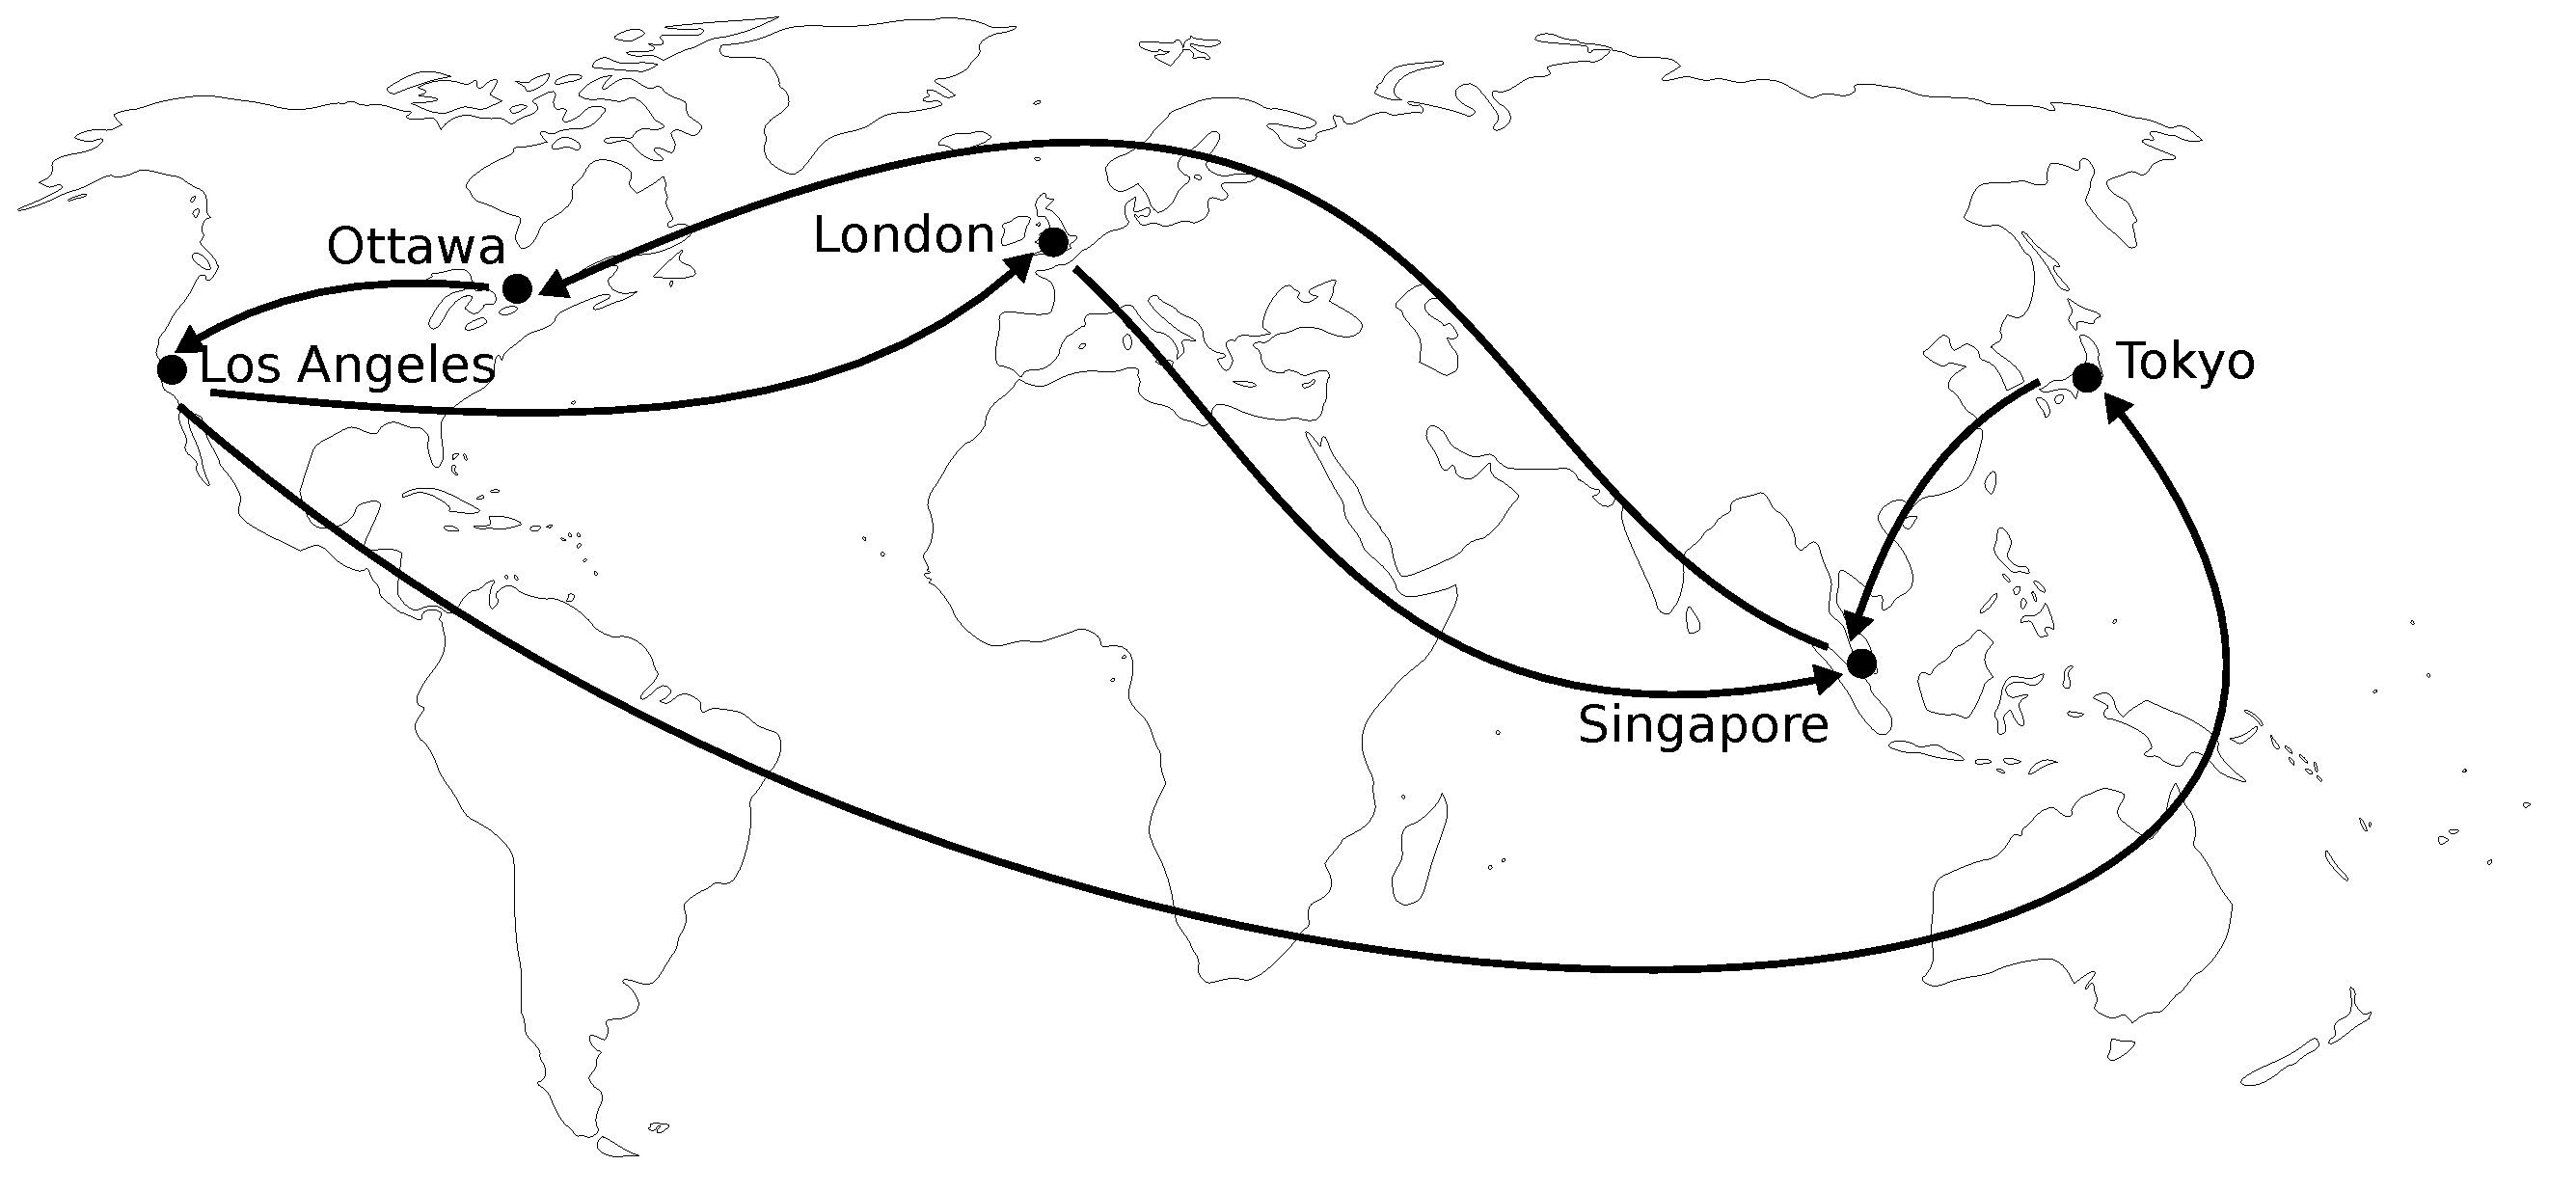
\includegraphics[height=2.5in]{flight_map.pdf}


\begin{enumerate}
	\item Write down a \emph{transition matrix} $A$ with entries $A_{i,j}$ which 
	are the number of ways to take exactly one flight from city $i$ to city $j$.
	\begin{enumerate}
		\item What do the diagonal entries tell you about the available flights?
		\item Should $A_{i,j} = A_{j,i}$? Explain.
	\end{enumerate}
	\item Write down a transition matrix $B$ with entries $B_{i,j}$ which are the 
	number of ways to take exactly two flights from city $i$ to city $j$.
	\begin{enumerate}
		\item Compute $A^2$ and compare with $B$.
		\item What information does the $1$st row of $A$ give you about flights?
		\item What information does the $2$nd column of $A$ give you about 
		flights?
		\item Based upon your last two answers what does the $1,2$ entry of 
		$A^2$ tell you about flights?
	\end{enumerate}
	\item Compute $A^3$ by any method.
		\begin{enumerate}
			\item Notice that the diagonal entries of $A$, $A^2$ and 
			$A^3$ are all zero. What is the first number $n$ so that 
			the diagonal entries of $A^n$ are non-zero?
			\item For what numbers $n$ do you expect $A^n$ to have a 
			non-zero diagonal entry? 
		\end{enumerate}
\end{enumerate}
\subsection*{Further Questions}
\begin{enumerate}[resume]
	\item Find a matrix $C$ with entries $C_{i,j}$ which are the number of ways to 
	fly from $i$ to $j$ in at most 3 flights. 
		\begin{enumerate}
			\item If you can fly at most three times, are all trips between 
			different cities possible? 
			\item Based on the trips of at most three flights which city 
			would make the best hub? (You may want to pick different cities
			for your outgoing and your incoming hubs.)
		\end{enumerate}
\end{enumerate}




%%%%%%%%%%%%%%%%%%%%%%%%%%%%%%%%%%%%%%%%%%%%%%%
% Challenge questions
%%%%%%%%%%%%%%%%%%%%%%%%%%%%%%%%%%%%%%%%%%%%%%%
\newpage
{
	\begin{center}
		{\bf \mthCourse, \mthTerm}\\ 
		{\bf Tutorial \#\mthTutorialNumber}\\
		{\bf \mthDate}
	\end{center}
}

\section*{Challenge questions}

A matrix $A$ is called \emph{primitive} if for large enough powers $A^n$
has all positive entries.
\begin{enumerate}[resume]

	\item Suppose that company A has 
	round-robin
	delivery service for 6 cities.  (That is there are routes from cities $1\to 2\to 3
	\to 4\to 5\to 6\to 1$.)  Let $A$ be the transition matrix for company A.
	Is $A$ primitive?
	\item Suppose there were a looping route from $1\to 1$ in addition.  Would $A$
	be primitive?
	\item Suppose a company B, with shipping routes $1\to 2\to 3\to 1$, buys 
	company A and so company B may now use its original routes or any of the newly
	aquired routes (Note, the self-loop is not included).  
	Let $B$ be the transition matrix for company B.  Is $B$ primitive?
	\item Suppose $C$ is a transition matrix for a shipping company with two round-robin
	shipping routes that intersect at exactly one city.  Give a condition on the 
	round-robin routes to ensure that $C$ is primitive.

\end{enumerate}



%%%%%%%%%%%%%%%%%%%%%%%%%%%%%%%%%%%%%%%%%%%%%%%
% TA instructions
%%%%%%%%%%%%%%%%%%%%%%%%%%%%%%%%%%%%%%%%%%%%%%%
\newpage
{\small
	\begin{center}
		{\bf \mthCourse, \mthTerm}\\ 
		{\bf Tutorial \#\mthTutorialNumber. Instructions for TAs}
	\end{center}
}

\subsection*{Objectives}

	We've been working hard at learning algorithms and matrix arithmetic.
	It's time to see matrices appear in an unexpected context and have some
	fun!

\subsection*{Hidden objectives}

	We've learned matrix multiplcation from one perspective, but it's
	time to think deeply about what is really going on combinatorically.

\subsection*{Suggestions}

\subsection*{Wrapup}
	Choose a question that most of the class has started but not yet finished,
	or a question that people particularly struggled with.

\subsection*{Solutions}
\begin{enumerate}
	\item
\end{enumerate}
	

\end{document}
